\section{Synthesis from Assume-Guarantee Contracts}
\label{sec:synthesis}

In this section we provide a summary of the formal background
that has already been established in previous work, regarding an algorithm that
is able to generate leaf-level component implementations using only the
information provided by the user through requirements expressed in the form of an
Assume-Guarantee contract. Our approach mainly supports the Linear Real
Arithmetic (LRA) theory, and to a certain extend the theory of integers (LIA),
mainly due to the limitations imposed by the underlying machinery. We
begin with a brief description of an Assume-Guarantee contract, and
move on to discuss the specifics of our program synthesis procedure,
which depends on our earlier work towards solving the problem of realizability
checking of contracts.
Finally, we enrich our formal definitions with an informal proof of the
algorithm's correctness in terms of the successfully synthesized
implementations.

\subsection{Assume-Guarantee Contracts}

In the context of requirements engineering, there have been a lot of proposed
ideas in terms of how requirements can be represented and expressed during
system design. One of the most popular ways to describe these requirements is through
the notion of an Assume-Guarantee contract, where the requirements are expressed
using safety properties that are split into two separate categories. The
\textit{assumptions} of the contract correspond to properties that restrict the
set of valid inputs a system can process, while the \textit{guarantees} dictate
what the system's behavior should be, using properties that precisely describe
the kinds of valid outputs that it may return to its environment.

\begin{figure}[H]
	\centering
	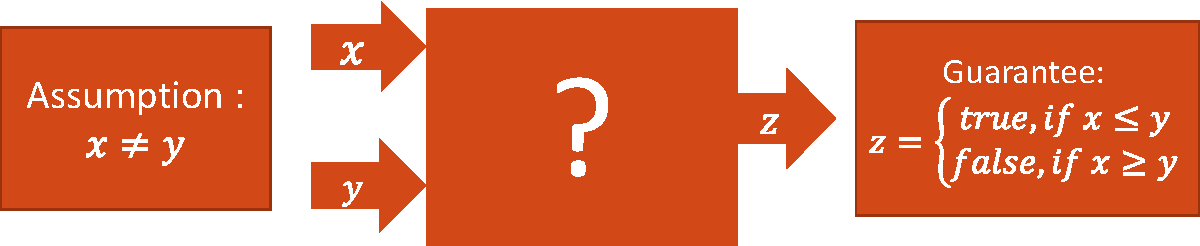
\includegraphics[width=\textwidth,height=\textheight,keepaspectratio]{real1-crop}    	
	\caption{Example of an Assume-Guarantee contract}
	\label{fg:example}
\end{figure}

As an illustrative example, consider the contract specified in
Figure~\ref{fg:example}. The component to be designed consists of two inputs,
$x$ and $y$ and one output $z$. If we restrict our example to the case of integer arithmetic,
we can see that the contract assumes that the inputs will never have the same value,
and requires that the component's output is a Boolean whose value depends on the comparison of the values of $x$ and $y$.
Also, notice that in the middle of the figure we depict the component using a
questionmark symbol. The questionmark is simply expressing the fact that during
the early stages of software development, the implementation is absent or exists only partially. This is particularly
important with respect to the problem of \textit{realizability}, where we try to
answer whether there exists an implementation that will satisfy the specific contract, under all circumstances. It is obvious that this is also
particularly important at the harder problem of \textit{program synthesis},
where the goal is to construct a witness of the contract's proof of realizability. In
Figure~\ref{fg:example}, one can easily answer that the contract is
\textit{realizable}, and therefore a synthesis procedure should be able to
provide us with an implementation. On the other hand, if we omit the contract's assumption, we can
safely say that the contract is \textit{unrealizable} as no implementation will
be able to provide a correct output in the case where $x=y$.

\subsection{Formal Preliminaries}
For the purposes of this paper, we are describing a system using the types
$state$ and $inputs$. Formally, an \textit{implementation}, i.e. a
\textit{transition system} can be described using a set of initial states $I(s)$ of type $state \rightarrow bool$, in addition to a transition relation $T(s,i,s')$ that
implements the contract and has the type $state \rightarrow inputs \rightarrow
state \rightarrow bool$.
 
An Assume-Guarantee contract can formally defined by two sets, a set of
\textit{assumptions} and a set \textit{guarantees}. The \textit{assumptions} $A$
impose constraints over the inputs, while the \textit{guarantees} $G$ used for
the corresponding constraints over the system's outputs and can be expressed as
two separate subsets $G_I$ and $G_T$, where $G_I$ defines the set of valid
initial states, and $G_T$ specifies the properties that need to be met during
each new transition between two states. Note that we do not necessarily expect
that a contract would be defined over all variables in the transition system,
but we do not make any distinction between internal state variables and outputs in the formalism.
This way, we can use state variables to, in some cases, simplify statements of guarantees.

\subsection{Realizability of Contracts}
The synthesis algorithm of this paper is essentially an extension on our
previous work on the realizabiility problem. Given the formal foundations above,
we expressed the problem of realizability using the notion of a state being
\textit{extendable}:

\begin{definition}[One-step extension]
\label{def:extend}
A state $s$ is extendable after $n$ steps, written $Extend_{n}(s)$, if
any valid path of length $n-1$ from $s$ can be extended in response to
any input. That is,
\begin{multline*}
\forall i_1, s_1, \ldots, i_n, s_n.\\ A(s, i_1) \land G_T(s, i_1, s_1)
\land \cdots \land
A(s_{n-1}, i_n) \land G_T(s_{n-1}, i_n, s_n)
\Rightarrow \\
\forall i.~ A(s_n, i) \Rightarrow \exists s'.~ G_T(s_n, i, s')
\end{multline*}
\end{definition}

The algorithm for realizability is using Definition~\ref{def:extend} in two
separate checks, that correspond to the two traditional cases exercised in
k-induction. For the \textit{BaseCheck}, we ensure that all initial states are
extendable in terms of any path of length $k<=n$, while the inductive step of
\textit{ExtendCheck} tries to prove that all valid states are extendable.
Therefore, we try to find the smallest $n$, for which the two following checks
hold:

\begin{equation}
\label{eq:sbcheck}
BaseCheck(n) = \forall k \leq n. (\forall s. G_I(s)
	  	\Rightarrow Extend_k(s))
\end{equation}

\begin{equation}
\label{eq:echeck}
ExtendCheck(n) = \forall s. Extend_n(s)
\end{equation}

The realizability checking algorithm has been used to effectively find cases
where the traditional consistency check failed to detect conflicts between
stated requirements in case studies of different complexity and importance. It
has also been formally verified using the Coq proof assistant in terms of its
soundness, for the cases where it reports that a contract is realizable.

\subsection{Program Synthesis from the proof of Realizability}

While the implemented algorithm on realizability provided us with meaningful
results during the verification of several contracts, the most apparent and
important outcome of this work was the fact that it could be effectively used as
the basis towards solving a more complex problem, which is that of
\textit{program synthesis}. Synthesis is defined as the process of automatically
deriving implementations, given a set of requirements specified by the user.
Since we are able to derive a proof regarding a contract's realizability,
i.e. a proof that an implementation exists for the specified
contract, we can use this proof in order to construct a witness
implementation that satisfies it. The limited power of SMT solvers
in terms of solving formulas containing nested quantifiers immediately ruled
out the prospect of using one as our primary synthesis tool. Fortunately, 
we are able to exploit our prior results in the scope of solving validity and 
Skolemizing $\forall\exists$-formulas (to be described in Sect.~\ref{sec:aeval}).

The idea behind our approach to solving the synthesis problem is
straightforward. Consider the checks~\ref{eq:sbcheck} and~\ref{eq:echeck} that
are used in the realizability checking algorithm. Both checks require
that the reachable states explored are extendable using
Definition~\ref{def:extend}.
The idea then is to decide if  $Extend_{n}(s)$ is valid and generate a witness 
for each of the $n$ times that we run \textit{BaseCheck} and a final witness 
for the inductive case in \textit{ExtendCheck}.

%GRIGORY: commented out the translation of A=> B => C into A /\ B => C since it is quite obvious

% Of course, 
%$Extend_{n}(s)$ as defined in~\eqref{def:extend} cannot
%be directly used for this purpose due to its form. This is not really an
%obstacle though, as we can rewrite the definition:
%
%\begin{multline*}
%\forall i_1, s_1, \ldots, i_n, s_n.\\ A(s, i_1) \land G_T(s, i_1, s_1)
%\land \cdots \land
%A(s_{n-1}, i_n) \land G_T(s_{n-1}, i_n, s_n)
%\Rightarrow \\
%\forall i.~ A(s_n, i) \Rightarrow \exists s'.~ G_T(s_n, i, s')
%\end{multline*}
%
%into an equivalent formula of the form $\forall \vec{x}.
%S(\vec{x}) \Rightarrow \exists \vec{y}. T(\vec{x},\vec{y})$ : 
%\begin{multline}
%	\label{ml:extendable2}
%		\forall i_1,s_1,\ldots,i_n,s_n,i. \\
%		A(s,i_1) \wedge G_T(s,i_1,s_1) \wedge \ldots \wedge
%		A(s_{n-1}, i_n) \wedge G_T(s_{n-1},i_n,s_n) \wedge A(s_n,i) \Rightarrow \\
%		\hspace{+2cm} \exists s'. G_T(s_n,i,s')
%	\end{multline}

\begin{figure}
\begin{small}
\begin{verbatim}
// for each variable in I or S,
//   create an array of size k.
//   then initialize initial state values
assign_GI_witness_to_S;
update_array_history;

// Perform bounded 'base check' synthesis
read_inputs;
base_check'_1_solution;
update_array_history;
...
read_inputs;
base_check'_k_solution;
update_array_history;

// Perform recurrence from 'extends' check
while(1) {
 read_inputs;
 extend_check_k_solution;
 update_array_history;
}
\end{verbatim}
\end{small}
\caption{Algorithm skeleton for synthesis}
\label{fig:algorithm}
\end{figure}

\noindent

Thus, we can construct the skeleton of an algorithm as shown in Figure~\ref{fig:algorithm}.  
We begin by creating an array for each input and history variable up to depth
$k$, where $k$ is the depth at which we found a solution to our realizability algorithm.
In each array, the zeroth element is the ``current'' value of the variable, the first element is the previous value, and the $(k-1)$'th value is the $(k-1)$-step previous value.
We then generate witnesses for each of the {\em BaseCheck} instances of
successive depth to describe the initial behavior of
the implementation up to depth $k$.  This process starts from the memory-free
description of the initial state ($G_I$).  There are two ``helper'' operations:
{\em update\_array\_history} shifts each array's elements one position forward
(the $(k-1)$'th value is simply forgotten), and {\em read\_inputs} reads the current values of inputs into the zeroth element of the input variable arrays.  Once the history is entirely initialized using the {\em BaseCheck} witness values, we enter a recurrence loop where we use the solution of the {\em ExtendCheck} to describe the next value of outputs.
 
 \andreas{Add proof of correctness here}


